\section{Formalization of Buddy Allocation Model}
The formalization of buddy allocation models consists of a specification for algorithms and proofs to properties for functional correctness. Compared with general buddy allocation algorithm, the difference in this paper is that we apply quartering way from Zephyr OS, an embedded system, for buddy allocation operations. This approach is more practical because it aims to pursue the efficiency. Since our specification requires a detailed description of the algorithms as well as the complex quartering way to describe, the foreseeable result is that it brings complexity to proofs than those abstract memory models.

For functional correctness, we try to answer these questions which are the basic of later properties: Do the algorithms pick out the most suitable block from all the available blocks? Do the algorithms correctly adjust the type of the relevant memory blocks after allocation and deallocation? How do the algorithms make sure to execute the merging operation after deallocation? How does the specification ensure the correctness of the quad-tree structure? What invariants does the specification preserve? Do the algorithms satisfy some security properties? Answering these questions contributes to the construction of a reliability memory system.

\subsection{Memory Model Specification}
The specification begins with the structure of a quad-tree.
\begin{align*}
(set:\ 'a)\ tree = &Leaf\ (L:\ 'a)\ | \\
&Node\ (LL:\ 'a\ tree)\ (LR:\ 'a\ tree)\ (RL:\ 'a\ tree)\ (RR:\ 'a\ tree) \\
&for\ map: tree\_map
\end{align*}
The quad-tree constructed by induction contains two pieces of information: the memory block type (indicated as \emph{ALLOC} and \emph{FREE} respectively); a address tag occupied by a memory block (indicated as \emph{ID}). The mapping function \textbf{tree.set} assists to collect the leaves from a tree. With the help of the block \textbf{type} and the function \textbf{get\_level} in a quad-tree, allocated leaves or free leaves from different levels can be gathered by \textbf{allocsets}, \textbf{freesets} and \textbf{freesets\_level}. All used \emph{ID} labels are in \emph{idset}. To create a new leaf, we have to pick up a new \emph{ID} to this new leaf by the strategy of \emph{SOME p. p} $\notin$ \emph{idset}. Later, we will prove that with this strategy, all leaves have different \emph{ID} labels.

Based on the above structure of a quad-tree, next we specify two operations with the buddy algorithms: \textbf{alloc} and \textbf{free}. For \emph{rsize} (the size of requested memory block) in allocation operation, there is a function that maps it to the level of the quad-tree and returns the most suitable level \emph{rlv}. The concept of \emph{most suitable level} will be proved in the next subsection. For the specification, we only use levels for both memory blocks in the quad-trees and requested memory blocks. And the smaller the level, the larger size the memory block.

\begin{definition} [existence of free blocks in level] \\
	exists\_freelevel blo\_set lv $\equiv$ $\exists$l. l $\leq$ lv $\wedge$ $\exists$b $\in$ blo\_set. freesets\_level b l $\ne$ $\emptyset$
\end{definition}

\begin{definition} [maximum level of free blocks] \\
	freesets\_maxlevel blo\_set lv $\equiv$ \\
	\phantom{x} \hspace{10pt} THE lmax. lmax $\leq$ lv $\wedge$ \\
	\phantom{x} \hspace{60pt} $\exists$b $\in$ blo\_set. freesets\_level b lmax $\neq$ $\emptyset$ $\wedge$ \\
	\phantom{x} \hspace{60pt} $\forall$l $\leq$ lv. $\exists$b $\in$ blo\_set. freesets\_level b l $\ne$ $\emptyset$ $\longrightarrow$ l $\leq$ lmax
\end{definition}

\begin{definition} [Allocation Operation] \\
	alloc blo\_set rlv $\equiv$ \\
	\phantom{x} \hspace{10pt} if exists\_freelevel blo\_set rlv then \\
	\phantom{x} \hspace{20pt} lmax = freesets\_maxlevel blo\_set rlv \\
	\phantom{x} \hspace{20pt} if lmax = rlv then \\
	\phantom{x} \hspace{30pt} btree = SOME b. b $\in$ blo\_set $\wedge$ freesets\_level b rlv $\ne$ $\emptyset$ \\
	\phantom{x} \hspace{30pt} l = SOME l. l $\in$ freesets\_level btree rlv \\
	\phantom{x} \hspace{20pt} else \\
	\phantom{x} \hspace{30pt} btree = SOME b. b $\in$ blo\_set $\wedge$ freesets\_level b lmax $\ne$ $\emptyset$ \\
	\phantom{x} \hspace{30pt} l = split (SOME l. l $\in$ freesets\_level btree lmax) (rlv - lmax) \\
	\phantom{x} \hspace{10pt} else False
\end{definition}

The first step of allocation is to check whether there is a quad-tree in \emph{blo\_set} (the memory pool tree collection), that has such free memory blocks whose level is less than or equal to \emph{rlv}. This step is done by \textbf{exists\_freelevel}, and if it returns \emph{False} then the allocation progress stops. Otherwise, the next step conducted by \textbf{freesets\_maxlevel} is to return the maximum level among all levels with free memory blocks. If the maximum level is equal to \emph{rlv}, then any free memory block in \emph{rlv} is to be allocated. If not, any free memory block in the maximum level is to be conducted by \textbf{split} showed in Fig. \ref{fig1} until free memory block in \emph{rlv} appears and then be allocated. The type of the assigned leaf is set to \emph{ALLOC}.

\begin{figure}
	\centering
	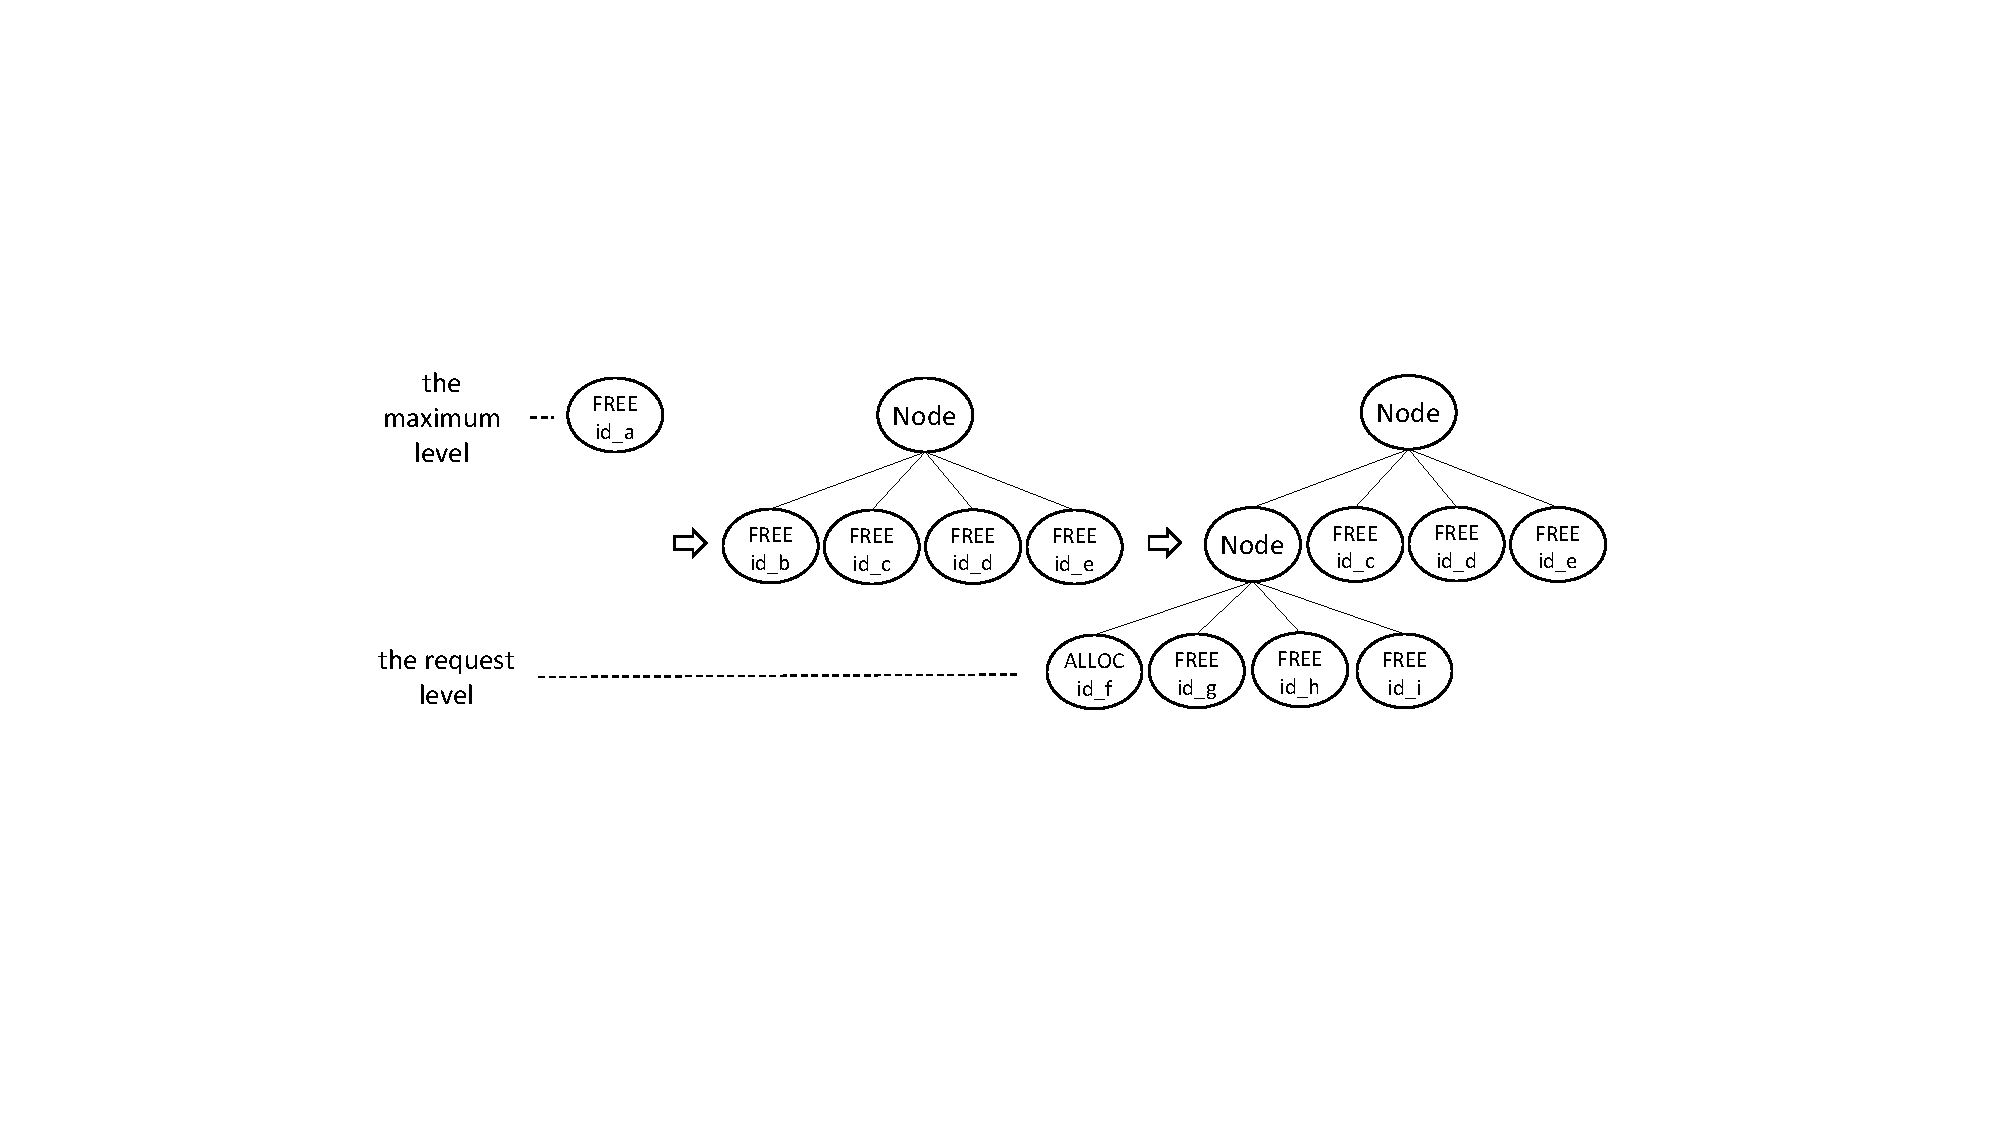
\includegraphics[width=1\textwidth]{fig1.pdf}
	\caption{The progress of dividing a free memory block}
	\label{fig1}
\end{figure}

\begin{definition} [Deallocation Operation] \\
	free blo\_set b $\equiv$ \\
	\phantom{x} \hspace{10pt} if $\exists$btree $\in$ blo\_set. b $\in$ tree.set btree then \\
	\phantom{x} \hspace{20pt} if type b = FREE then False \\
	\phantom{x} \hspace{20pt} else btree = THE t. t $\in$ blo\_set $\wedge$ b $\in$ tree.set t \\
	\phantom{x} \hspace{40pt} merge (reset btree b FREE) \\
	\phantom{x} \hspace{10pt} else False
\end{definition}

The deallocation progress firstly checks whether there is a quad-tree in \emph{blo\_set} that the occupied memory block to be released belongs to this tree. If there is no such tree, the procedure returns \emph{False}. Next, if the type of the occupied memory block is \emph{FREE}, the progress also returns \emph{False}. When all conditions are met, the memory block is returned to the tree it belongs to, thereafter merging operation is executed. The merging operation is to combine all free memory blocks that belong to the same parent tree showed in Fig. \ref{fig2}.

\begin{figure}
	\centering
	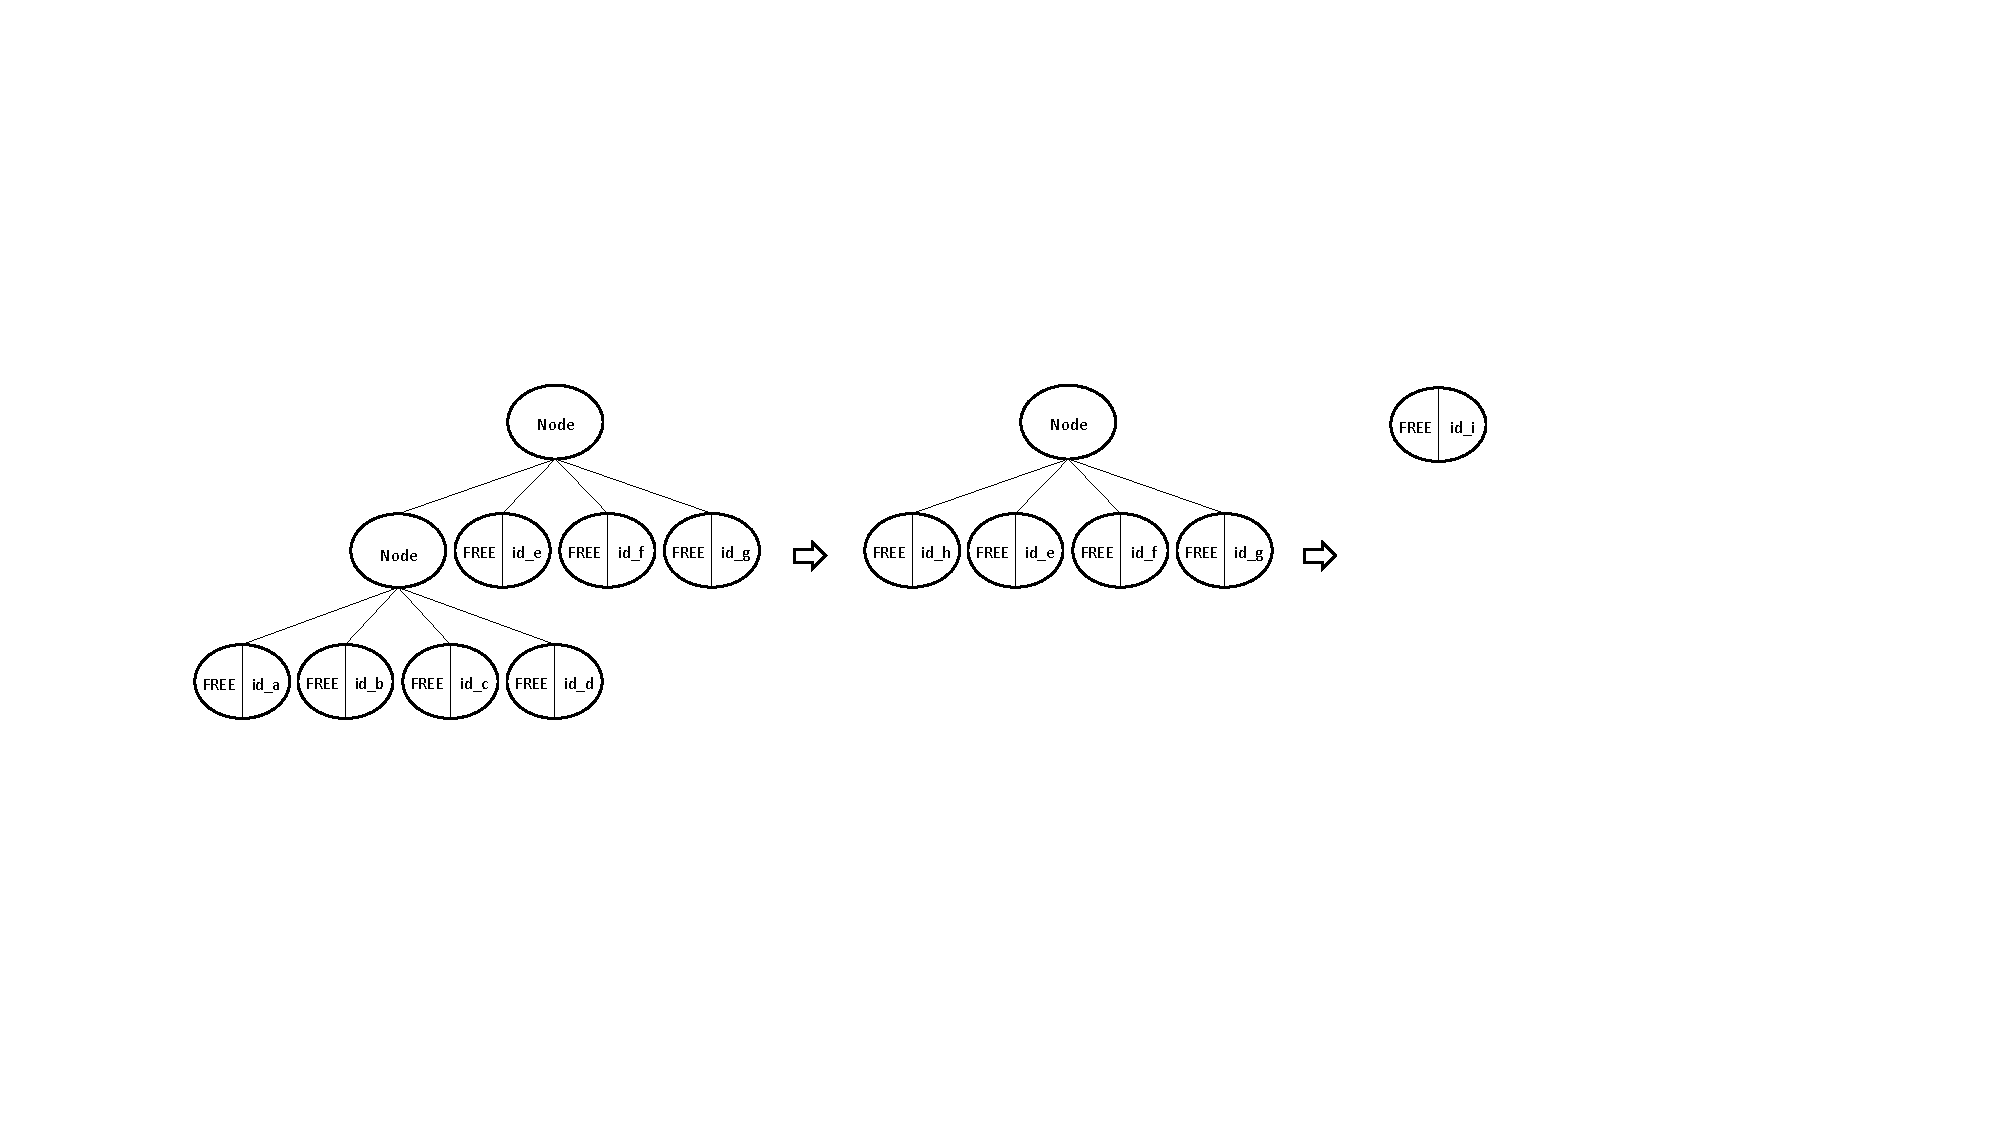
\includegraphics[width=1\textwidth]{fig2.pdf}
	\caption{The progress of merging all free memory blocks}
	\label{fig2}
\end{figure}

Owing to space constraints, the \emph{split} and the \emph{merge} operations constructed by induction are not described in detail. At this point, we have done the specification for the buddy memory algorithms. Next, we are going to verify the properties to guarantee the functional correctness of this specification.

\subsection{Memory Model Properties}
Once the specification is finished, the preconditions $\&$ postconditions for functions as well as the invariants are to be raised up to ensure the functional correctness of the specification. We give preconditions and postconditions in the first place.

The following Def. \ref{pp1} gives such an implication: if there is not a quad-tree in \emph{blo\_set} that has free memory blocks whose level is less than or equal to \emph{rlv}, nothing is to be changed because of the allocation failure.

\begin{definition} [Allocation Failure] \\
	$\neg$ exists\_freelevel blo\_set rlv $\longrightarrow$ fst (alloc blo\_set rlv) = blo\_set
	\label{pp1}
\end{definition}

Then Def. \ref{pp2} and Def. \ref{pp3} respectively describe the block to be allocated no longer belongs to the free sets and is part of allocated sets during the direct allocation process.

\begin{definition} [Freesets for Direct Allocation] \\
	exists\_freelevel blo\_set rlv $\wedge$ freesets\_maxlevel blo\_set rlv = rlv $\longrightarrow$ \\
	\phantom{x} \hspace{10pt} $\exists$l. l $\in$ freesets blo\_set $\wedge$ l $\notin$ freesets fst (alloc blo\_set rlv) $\wedge$ \\
	\phantom{x} \hspace{10pt} freesets blo\_set = freesets fst (alloc blo\_set rlv) $\cup$ $\lbrace$l$\rbrace$
	\label{pp2}
\end{definition}

\begin{definition} [Allocsets for Direct Allocation] \\
	exists\_freelevel blo\_set rlv $\wedge$ freesets\_maxlevel blo\_set rlv = rlv $\longrightarrow$ \\
	\phantom{x} \hspace{10pt} $\exists$l. l $\notin$ allocsets blo\_set $\wedge$ l $\in$ allocsets fst (alloc blo\_set rlv) $\wedge$ \\
	\phantom{x} \hspace{10pt} allocsets fst (alloc blo\_set rlv) = allocsets blo\_set $\cup$ $\lbrace$l$\rbrace$
	\label{pp3}
\end{definition}

Next Def. \ref{pp4} says that a new block created from splitting a bigger block is allocated and belongs to the allocated sets during indirect allocation, which means \emph{split} operation is needed.

\begin{definition} [Allocsets for Indirect Allocation] \\
	exists\_freelevel blo\_set rlv $\wedge$ freesets\_maxlevel blo\_set rlv $\neq$ rlv $\longrightarrow$ \\
	\phantom{x} \hspace{10pt} $\exists$l. l $\notin$ allocsets blo\_set $\wedge$ l $\in$ allocsets fst (alloc blo\_set rlv) $\wedge$ \\
	\phantom{x} \hspace{10pt} allocsets fst (alloc blo\_set rlv) = allocsets blo\_set $\cup$ $\lbrace$l$\rbrace$
	\label{pp4}
\end{definition}

The next two Def. \ref{pp5} and Def. \ref{pp6} guarantee nothing to be changed during the deallocation process because of the non-existence of such a quad-tree that the block to be released belongs to or the type of the block to be freed is \emph{FREE}.

\begin{definition} [Deallocation failure 1] \\
	$\nexists$btree $\in$ blo\_set. b $\in$ tree.set btree $\longrightarrow$ fst (free blo\_set b) = blo\_set
	\label{pp5}
\end{definition}

\begin{definition} [Deallocation failure 2] \\
	$\exists$btree $\in$ blo\_set. b $\in$ tree.set btree $\wedge$ type b = FREE $\longrightarrow$ \\
	\phantom{x} \hspace{10pt} fst (free blo\_set b) = blo\_set
	\label{pp6}
\end{definition}

The last Def. \ref{pp7} tells that the block to be deallocated does not belong to allocated sets any more.

\begin{definition} [Allocsets for Deallocation Success] \\
	$\exists$btree $\in$ blo\_set. b $\in$ tree.set btree $\wedge$ type b $\neq$ FREE $\longrightarrow$ \\
	\phantom{x} \hspace{10pt} allocsets blo\_set = allocsets fst (free blo\_set b) $\cup$ $\lbrace$b$\rbrace$
	\label{pp7}
\end{definition}

After giving these definitions for preconditions and postconditions, we try to prove that our buddy allocation specification satisfies them so that it meets the functional expectations. The first theorem we prove as follows.

\begin{theorem}
The buddy allocation specification satisfies all the preconditions and postconditions above.
\end{theorem}

\begin{proof}
	All parts can be formally proved by induction on the type of a quad-tree, including leaf and node types. And the proofs on node type can be conducted by another induction which is on the height of the derivation.
\end{proof}

Through preconditions and postconditions, the specification can be proved that it partly follows the expectations of the algorithms. Next to guarantee that the algorithms pock out the most suitable block, two properties have to be proved: 1. the correctness of the mapping from the request memory block size to the level of the quad-tree. 2. the correctness of the quad-tree hierarchical structure. Here are these two properties.

\begin{definition} [Mapping Request Sizes to Allocation Levels] \\
	output\_level blo\_list rsize $\equiv$ THE l. l $<$ L blo\_list $\wedge$ rsize $\le$ blo\_list ! l $\wedge$ \\
	\phantom{x} \hspace{10pt} (L blo\_list $>$ 1 $\wedge$ l $<$ L blo\_list - 1) $\longrightarrow$ rsize $>$ L blo\_list ! (l+1)
\end{definition}

Static linked list \emph{blo\_list} is used to store the size of block for each level in a quad-tree. For example, the size of root is 1024\emph{M} and the first level is 256\emph{M}, then \emph{blo\_list}!0 is equal to 1024 and \emph{blo\_list}!1 is 256. The \emph{blo\_list} is a strictly decreasing list. Function \textbf{L} is used to get the length of a list. As mentioned above, the smaller the level, the larger size the memory block. The most suitable block means that its size has to be greater than or equal to the size of request block, and there is no smaller block that meets this condition. Through this definition, the most suitable block is picked up from \emph{blo\_list}, and then mapped to the correct level of the quad-tree by the index of \emph{blo\_list}. Some lemmas ensure the correctness of this definition.

\begin{lemma}
	L blo\_list $>$ 0 $\wedge$ rsize $\leq$ blo\_list ! (L blo\_list - 1) $\longrightarrow$ output\_level blo\_list rsize = L blo\_list - 1
\end{lemma}

\begin{lemma}
	L blo\_list $>$ 1 $\wedge$ l $<$ L blo\_list - 1 $\wedge$ rsize $\leq$ blo\_list ! l $\wedge$ rsize $>$ blo\_list ! (l + 1) $\longrightarrow$ output\_level blo\_list rsize = l
\end{lemma}

\begin{proof}
	By unfolding the definition of output\_level, two aspects including existence and uniqueness have to be proved for the notion THE. The first part existence can be proved by the given assumptions. The remaining part uniqueness can be proved by the strictly decreasing blo\_list.
\end{proof}

Next, we introduce a lemma alone to prove the correctness of a quad-tree structure from the aspect of its levels. The \textbf{root} checks whether the tree is a root tree and \textbf{child} gives us all immediate child nodes.

\begin{lemma}
	(root btree $\longrightarrow$ get\_level btree = 0) $\wedge$ (get\_level btree = l $\wedge$ l $\geq$ 0 $\wedge$ chtree $\in$ child btree $\longrightarrow$ get\_level chtree = l + 1)
\end{lemma}

\begin{proof}
	This lemma can be formally proved by induction on the height of the derivation.
\end{proof}

Until now, we have already proved the correctness of the mapping operation and the hierarchical structure of a quad-tree. Then we can deduce the following theorem to guarantee the property of picking out the most suitable memory block.

\begin{theorem}
	The buddy allocation specification picks out the most suitable memory block and operates on the correct level in a quad-tree.
\end{theorem}

The algorithms are designed to avoid the fragmentation by merging operation which is invoked in the process of deallocation. Whether this operation is executed correctly can not be proved from the surface. In order to prove this property, we still start from the structural correctness of the quad-tree. Considering the fact that there is not such a node whose four child nodes are all leaves and their types are \emph{FREE} after merging operation, a definition to check whether a tree is like this can be constructed as follows. The \textbf{leaf} is to check whether the tree is a leaf.

\begin{definition} [Four Free Leaves Belong to The Same Node] \\
	is\_FFL btree $\equiv$ $\forall$chtree $\in$ child btree. leaf chtree $\wedge$ type chtree = FREE
\end{definition}

Fig. \ref{fig2} can explain this definition well. Just like the subtree in the lower left corner of the first picture, four child nodes are all leaves and their types are \emph{FREE}. Therefore, merging operation is necessary during the progress of deallocation to handle this situation. The following are the lemmas that ensure the non-existence of such \emph{FFL} trees after allocation and deallocation operations if non-existence of such trees in preconditions.

\begin{lemma}
	$\forall$b $\in$ blo\_set. $\neg$ is\_FFL b $\longrightarrow$ $\forall$b $\in$ fst (alloc blo\_set rlv). $\neg$ is\_FFL b
\end{lemma}

\begin{lemma}
	$\forall$b $\in$ blo\_set. $\neg$ is\_FFL b $\longrightarrow$ $\forall$b $\in$ fst (free blo\_set b). $\neg$ is\_FFL b
\end{lemma}

\begin{proof}
	Apply cases to these two lemmas after folding the definitions of allocation and deallocation operations. For each cases, they can be proved by induction on the height of the derivation.
\end{proof}

After memory initialization, assuming that all blocks to be allocated are the original ones which are not split, this beginning of the moment satisfies non-existence of \emph{FFL} trees among all quad-trees because all available blocks are seen as root trees. This assertion satisfies the assumptions in the implication expressions above. Therefore, through any execution orders of allocation and deallocation operations, the whole memory system satisfies non-existence of the \emph{FFL} trees. We have this theorem as follows.

\begin{theorem}
	The buddy allocation specification guarantees non-existence of FFL trees among all quad-trees.
\end{theorem}

In the end, we prove two significant properties: memory isolation and non-leakage. The first one is to prove non-existence of the overlap in the address spaces. Isolation in address spaces makes sure domains' memory blocks are not maliciously overwritten. Memory leakage means that available memory blocks (including occupied and free blocks) are getting less and less. Then non-leakage is to protect the integrity of address spaces.

Now we begin with the memory isolation. For the specification level, we provisionally use \emph{ID} to represent a contiguous addresses for a memory block. When we introduce real addresses into the specification, two things have to be proved: 1. the correctness of mapping function between a \emph{ID} and a true range of address; 2. the one-to-one uniqueness between them. In this paper, we are not going to introduce real addresses and we assume the above properties are all correct. Therefore, in this specification, isolation in address spaces means that all \emph{IDs} that leaves bring are different. What we prove to guarantee the difference of \emph{IDs} is the strategy of creating a new leaf that has been already introduced in the subsection 3.1.

The following definition tells that there are no two leaves with the same \emph{ID}. The \textbf{ID} gives the id the leaf brings. Firstly, we pick up any quad-tree \emph{b} from the tree collection \emph{blo\_set}. Then we select any leaf \emph{l} from this quad-tree. Our criterion is that there is not such a leaf \emph{l'} picked up from any quad-tree that is different from \emph{l} but has the same \emph{ID} with \emph{l}.

\begin{definition} [Different IDs] \\
	is\_different blo\_set $\equiv$ $\forall$b $\in$ blo\_set. $\forall$l $\in$ tree.set b. ($\nexists$l'. l' $\in$ tree.set (SOME b. b $\in$ blo\_set) $\wedge$ l' $\ne$ l $\wedge$ ID l' = ID l)
\end{definition}

Below are two lemmas that ensure this property holds during the procedures of allocation and deallocation if it holds in preconditions.

\begin{lemma}
	is\_different blo\_set $\longrightarrow$ is\_different fst (alloc blo\_set rlv)
\end{lemma}

\begin{lemma}
	is\_different blo\_set $\longrightarrow$ is\_different fst (free blo\_set b)
\end{lemma}

\begin{proof}
	Firstly apply cases to these two lemmas after folding the definitions of allocation and deallocation operations. Then for each cases, they can be proved by induction on the height of the derivation.
\end{proof}

With above lemmas of different \emph{IDs}, we can ensure all \emph{IDs} are different by using our strategy to create a new leaf. The following is the theorem that says this.

\begin{theorem}
	The buddy allocation specification ensures all IDs of leaves are different.
\end{theorem}

Finally, combined with the assumptions that mapping function between a \emph{ID} and a true range of address is correct, memory isolation in addresses can be proved.

Next is for the non-leakage of blocks. Result from we use the quad-tree structure and map all the memory blocks into the leaves of these trees, thence the non-leakage means that all the leaves (including occupied and free leaves) are in use. If we can infer that the quad-tree always maintains correct structure from the aspect of a relation between the number of nodes and leaves, then we can prove that all the leaves are in use and none leaf is forgotten. The first step is to prove a relation between the number of nodes and leaves in a quad-tree. Functions \textbf{Leaf} and \textbf{Node} give all the leaves and nodes in a quad-tree \emph{b}.

\begin{lemma}
	q-tree b: Num (Leaf b) = Num (Node b) $\times$ 3 + 1
\end{lemma}

\begin{proof}
	This lemma can be formally proved by induction on the type of quad-tree b, including leaf and node types. If quad-tree b is a leaf which means it is also a root, then the number of leaves is 1 and the number of nodes is 0. The lemma can be proved. If quad-tree b is a node with the inductive assumptions that this relation in the number of leaves and nodes holds for all the subtrees in b, this lemma still can be proved because of the quad-tree structure of b itself.
\end{proof}

Having established this relation, we use the following two lemmas to guarantee all the quad-trees during the procedures maintain this relation in the number of leaves and nodes.

\begin{lemma}
	$\forall$b $\in$ blo\_set. q-tree b $\longrightarrow$ $\forall$b $\in$ fst (alloc blo\_set rlv). q-tree b
\end{lemma}

\begin{lemma}
	$\forall$b $\in$ blo\_set. q-tree b $\longrightarrow$ $\forall$b $\in$ fst (free blo\_set b). q-tree b
\end{lemma}

\begin{proof}
	Fold the definitions of allocation and deallocation operations firstly. Then apply cases to these two lemmas. For each cases, they can be proved by induction on the height of the derivation.
\end{proof}

In the end, we can prove that all quad-trees holds this relation in the number of leaves and nodes. That is to say all leaves (including occupied and free leaves) are in use. Then considering the fact that all blocks are mapped into the leaves of these trees, we can ensure non-leakage of memory in our specification.

\begin{theorem}
	The buddy allocation specification guarantees any tree is a q-tree.
\end{theorem}

To sum up, in this section we introduce the quad-tree structure to simulate memory because of the buddy allocation algorithms. Then we give a specification for the algorithms including \textbf{alloc} and \textbf{free} operations. After that, we give proofs for functional correctness including preconditions and postconditions, the most suitable memory block, non-existence of the \emph{FFL} trees, memory isolation and non-leakage. Through these efforts, we give a functionally correct buddy memory model.